\RequirePackage{silence}
\WarningFilter{hyperref}{Token not allowed}
\WarningFilter{microtype}{tracking amount}
\WarningFilter{chessfss}{\comment already}
% LaTeX: More Than Just Academic Papers and Journals
%
% Copyright Lim Lian Tze 2011-2016 (liantze@gmail.com) 
% Beamer presentation slides for a talk at the Malaysian Open Source Conference 
% 2011 (MOSC 2011 http://www.mosc.my/)
%
% http://liantze.penguinattack.org/latextypesetting.html
%
% This work is licensed under a Creative Commons Attribution-NonCommercial-
% ShareAlike 3.0 Unported License (http://creativecommons.org/licenses/by-nc-sa/3.0/).
%

%\pdfminorversion=5
%\pdfobjcompresslevel=3 
%\pdfcompresslevel=9

% Full presentation (with overlays, animated bullet items etc)
\documentclass[aspectratio=169,xcolor={x11names,svgnames,dvipsnames}]{beamer}

% Transparency mode (no overlays)
%\documentclass[xcolor={x11names,svgnames,dvipsnames},trans]{beamer}

% n-up handout mode
% \documentclass[xcolor={x11names,svgnames,dvipsnames},handout]{beamer}

\usepackage{pgfpages}
\usepackage{qrcode}

\usepackage[british]{babel}
\usepackage[utf8]{inputenc}
\usepackage[T1]{fontenc}
\usepackage{lmodern}
% \usepackage[linesnumbered,lined,commentsnumbered]{algorithm2e}
\usepackage[lined]{algorithm2e}
\usepackage{graphicx}

%% Glossy pretty look for the presentation and transparency (w/o overlays and animations) versions!
\mode<beamer|trans>{
\useoutertheme[glossy]{wuerzburg}
\useinnertheme[shadow,outline]{chamfered}
\usecolortheme{shark}
}
\setbeamertemplate{navigation symbols}{}
\setbeamertemplate{frametitle continuation}[from second][(cont'd)]
\usefonttheme[stillsansseriftext,stillsansserifsmall]{serif}

%% Save up on ink for the 4-up handouts
\mode<handout>{
\useoutertheme{wuerzburg}
\useinnertheme[outline]{chamfered}
%\pgfpagesuselayout{4 on 1}[a4paper, landscape, border shrink=10mm]
\pgfpagesuselayout{2 on 1}[a4paper, border shrink=10mm]
\pgfpageslogicalpageoptions{1}{border code=\pgfstroke}
\pgfpageslogicalpageoptions{2}{border code=\pgfstroke}
%\pgfpageslogicalpageoptions{3}{border code=\pgfstroke}
%\pgfpageslogicalpageoptions{4}{border code=\pgfstroke}
\setbeamercolor{structure}{fg=black}
\setbeamercolor{alerted text}{fg=black}
}

\mode<presentation>{\AtBeginSection[]{%
\begin{frame}
\frametitle{Contents}
\tableofcontents[currentsection]
\end{frame}}}

\usepackage[T1,safe]{tipa}
\usepackage{microtype}
\usepackage[utf8]{inputenc}
\usepackage[T1]{fontenc}
\usepackage{libertine}
\usepackage[scaled=.77]{beramono}
\SetTracking{encoding=*}{-39}

\usepackage{relsize,tabularx}
\usepackage{hologo,textcomp}
\usepackage{comment}
\usepackage[skaknew]{chessboard,skak}
\usepackage{multicol,booktabs}
\usepackage{listings}
\lstset{upquote,keepspaces=true,columns=spaceflexible,
basicstyle=\ttfamily\scriptsize,%
breaklines=true,breakindent=0pt,xleftmargin=0pt, xrightmargin=6pt,%
language=[LaTeX]TeX, texcsstyle=*\bfseries\color{Maroon}, commentstyle=\sffamily\itshape\smaller\color{SeaGreen4},
emphstyle=\bfseries\color{RoyalBlue3},escapechar={:},
emphstyle={[2]{\bfseries\color{Sienna2}}},
postbreak=\mbox{{\smaller\color{gray}$\hookrightarrow$}}
}

\mode<handout>{
   \lstset{
   texcsstyle=*\bfseries, commentstyle=\sffamily\itshape\smaller,
   emphstyle=\bfseries,escapechar={:},
   emphstyle={[2]{\bfseries}},
   emphstyle={[3]{\bfseries}},
   postbreak=\mbox{{\smaller$\hookrightarrow$}}
   }
}

\makeatletter
\lst@CCPutMacro\lst@ProcessOther {"2D}{\lst@ttfamily{-{}}{-{}}}
\@empty\z@\@empty
\makeatother


\usepackage{tikz}
\usepackage{pgfgantt}
\usetikzlibrary{shapes,arrows,positioning,matrix,chains,fit}
\usetikzlibrary{backgrounds}

\usepackage[caption=false,font=footnotesize]{subfig}
\usepackage{blindtext}
\usepackage{amssymb}
\usepackage{amsthm}
\usepackage{amsmath}
\usepackage{mathtools}
\usepackage{changepage}
\usepackage{color}
\usepackage{colortbl}
\usepackage{hhline}
\usepackage{array}
\usepackage{multicol,multirow}
\usepackage[version=3]{mhchem}
\usepackage{chemfig}
\usepackage{expex,qtree}
% \usepackage{texshade}
\usepackage[detect-all]{siunitx}
% \usepackage[siunitx]{circuitikz}
\usepackage{smartdiagram}
\usepackage{bytefield}
\usepackage{fancybox}
\usepackage{graphicx}
\usepackage{color}
\usepackage{epsfig}

\usepackage{epstopdf}
\usepackage{multimedia}
%\usepackage[latin1]{inputenc}
%\usepackage{indentfirst}
%\usepackage[brazil]{babel}
\usepackage{mdframed}
\usepackage{multirow}
\usepackage{booktabs}
\usepackage{epstopdf}
\usepackage{xspace}
\bibliographystyle{unsrt}
% \usepackage{pstricks,pst-barcode}
% \usepackage{auto-pst-pdf}

\definecolor{light-gray}{rgb}{0.98, 0.99, 0.99}
\definecolor{light-orange}{rgb}{0.95, 0.95, 0.99}
\definecolor{light-green}{rgb}{0.90,0.95,0.90}
\definecolor{sepia}{rgb}{0.44, 0.26, 0.08}
\definecolor{olive}{rgb}{0.5, 0.5, 0.0}
\definecolor{safe1}{rgb}{0.38, 0.38, 0.38}
\definecolor{safe2}{rgb}{0.74, 0.74, 0.74}
\definecolor{safe3}{rgb}{0.90, 0.90, 0.90}
%\definecolor{ceruleanblue}{rgb}{0.16, 0.32, 0.75}
%\definecolor{cornellred}{rgb}{0.7, 0.11, 0.11}
%\definecolor{darkpastelgreen}{rgb}{0.01, 0.75, 0.24}
%\definecolor{green(pigment)}{rgb}{0.0, 0.65, 0.31}


% power supply
%
% paragraph, up 100 words
% cfp@splintercon.net
% today
%
% presentation by friday

\newcolumntype{L}{>{\scriptsize}l}
\newcolumntype{C}{>{\scriptsize}c} % define a new column type for \tin

\newcolumntype{x}{>{\columncolor{light-gray}}C}
\newcolumntype{y}{>{\columncolor{white}}C}
\newcolumntype{z}{>{\columncolor{light-orange}}C}


\usepackage{pgfplots}
\pgfplotsset{compat=1.12}
\usepackage{cwpuzzle}
\usepackage{gchords,guitar}
\usepackage{spreadtab}
\usepackage{ccicons}
\usepackage{marvosym}
\usepackage{upgreek}
\usepackage{adforn}
% \ifpdf
\pdfmapfile{+webo.map}
% \fi
\newcommand{\wb}[1]{{\usefont{U}{webo}{xl}{n}#1}}
\usepackage{bookmark}

\usepackage{graphicx}

\usepackage{epigraph}
\setlength{\epigraphwidth}{1\textwidth}

\setlength\fboxsep{0pt}


\author[Rafael Diniz]{\texorpdfstring{\textcolor{blue}{Rafael Diniz} \\
%{Rhizomatica} \\
%{Digital Telecommunication in HF band - WWWAN - World-Wide Wireless Area Network}\\
\url{rafael@rhizomatica.org}}{Rafael Diniz}}
\title{Building an Autonomous World-Wide HF Band Wireless Network}
\subtitle{
\texorpdfstring{ %(\textsc{UT--Dallas})\\%
\hrulefill\ \adforn{57}\thickspace\wb{.}\thickspace\adforn{29}\ \hrulefill}
%{}
}

\titlegraphic{\includegraphics[width=.4\textwidth]{logo.png} \ \ \ \ \ \  \\}
\date[2024]{}
\hypersetup{%
pdfauthor={Rafael Diniz}, %% the "author" field from above includes garbage code...
%pdfkeywords={latex,features,publicity,preview}
}
\begin{document}

\begin{frame}[plain]
\maketitle
\end{frame}


\begin{frame}
\begin{center}
  \includegraphics[width=.9\columnwidth]{hermes.png}
\end{center}
\end{frame}

% move information around worldwide communication
% safe / security / non traceable
% stealth transmission / non-line-of-sight
% most resilient and secure communication

\begin{frame}{Introduction - HERMES}

  \begin{itemize}
  \item HERMES was born from the struggle to provide
  telecommunication access to indigenous and riverside
  communities in the Amazon rainforest.

  \item For decades many communities in Amazon, Central Africa, and other
  places without telecom infrastructure relied on analog SSB HF radios
  for long range voice communication.

  \item While HF telecom was once the most advanced long range
  wireless communication technology, nowadays its civil use is
  restricted to enthusiasts and isolated communities, and is
  technologically stuck in the 60's. HERMES aims to push forward
  civil HF telecom state-of-the-art.

  \item HERMES provides a digital telecommunication solution for HF
  which allows the deployment of regional and worldwide autonomous
  networks without any pre-existing telecom infrastructure.

  \end{itemize}

\end{frame}

% Slide 2
\begin{frame}{Introduction - The HF Band}

  \begin{itemize}
  \item Defined by ITU as the electromagnetic spectrum between 3 MHz and 30 MHz
  \item The HF band allows very wide coverage thanks to the Earth's ionosphere reflective
    properties for the HF band (MF too)
  \item The propagation type of a signal that reflects or refracts in the ionosphere is called
    skywave
  \item HF is the most resilient telecommunication media and is very hard
  to track a transmission
  \end{itemize}

  \begin{center}
    \vspace{-0.1cm}
  \includegraphics[width=.5\columnwidth]{bands.png}
\end{center}

\end{frame}


\begin{frame}{Introduction - Skywave propagation}

  \begin{itemize}
  \item The Ionosphere is located in the upper atmosphere, from 80 up 1000 km in altitude
  \item Skywave can be used for relativelly short distances, up to hundreds of kilometers, and
    long distances communication, to any point on Earth
  \end{itemize}


\begin{center}
  \includegraphics[width=.48\columnwidth]{skywave.jpeg}
%  \includegraphics[width=.45\columnwidth]{ionosfera.png}
  \includegraphics[width=.5\columnwidth]{skywave.jpg}

\end{center}

\end{frame}


\begin{frame}{Introduction - HF Antenna}

  \begin{itemize}
  \item Frequencies: between 3 MHz and 10 MHz typical for regional coverage
  \item Antennas (Example): dipole or folded dipole typical, in horizontal or inverted V layout
  \end{itemize}


  \begin{center}
    \includegraphics[width=.39\columnwidth]{antena.jpeg}
    \includegraphics[width=.51\columnwidth]{antena.jpg}
  \end{center}

\end{frame}

\begin{frame}{HERMES History}

  \begin{itemize}
    \item Fonias Juruá (2015): Stock HF SSB transceiver connected to a box with radio interface, Rasperry Pi and touch screen. Modem used is HamDRM (DRM narrowband).
  \end{itemize}
% \vspace{-0.5cm}
\begin{center}
  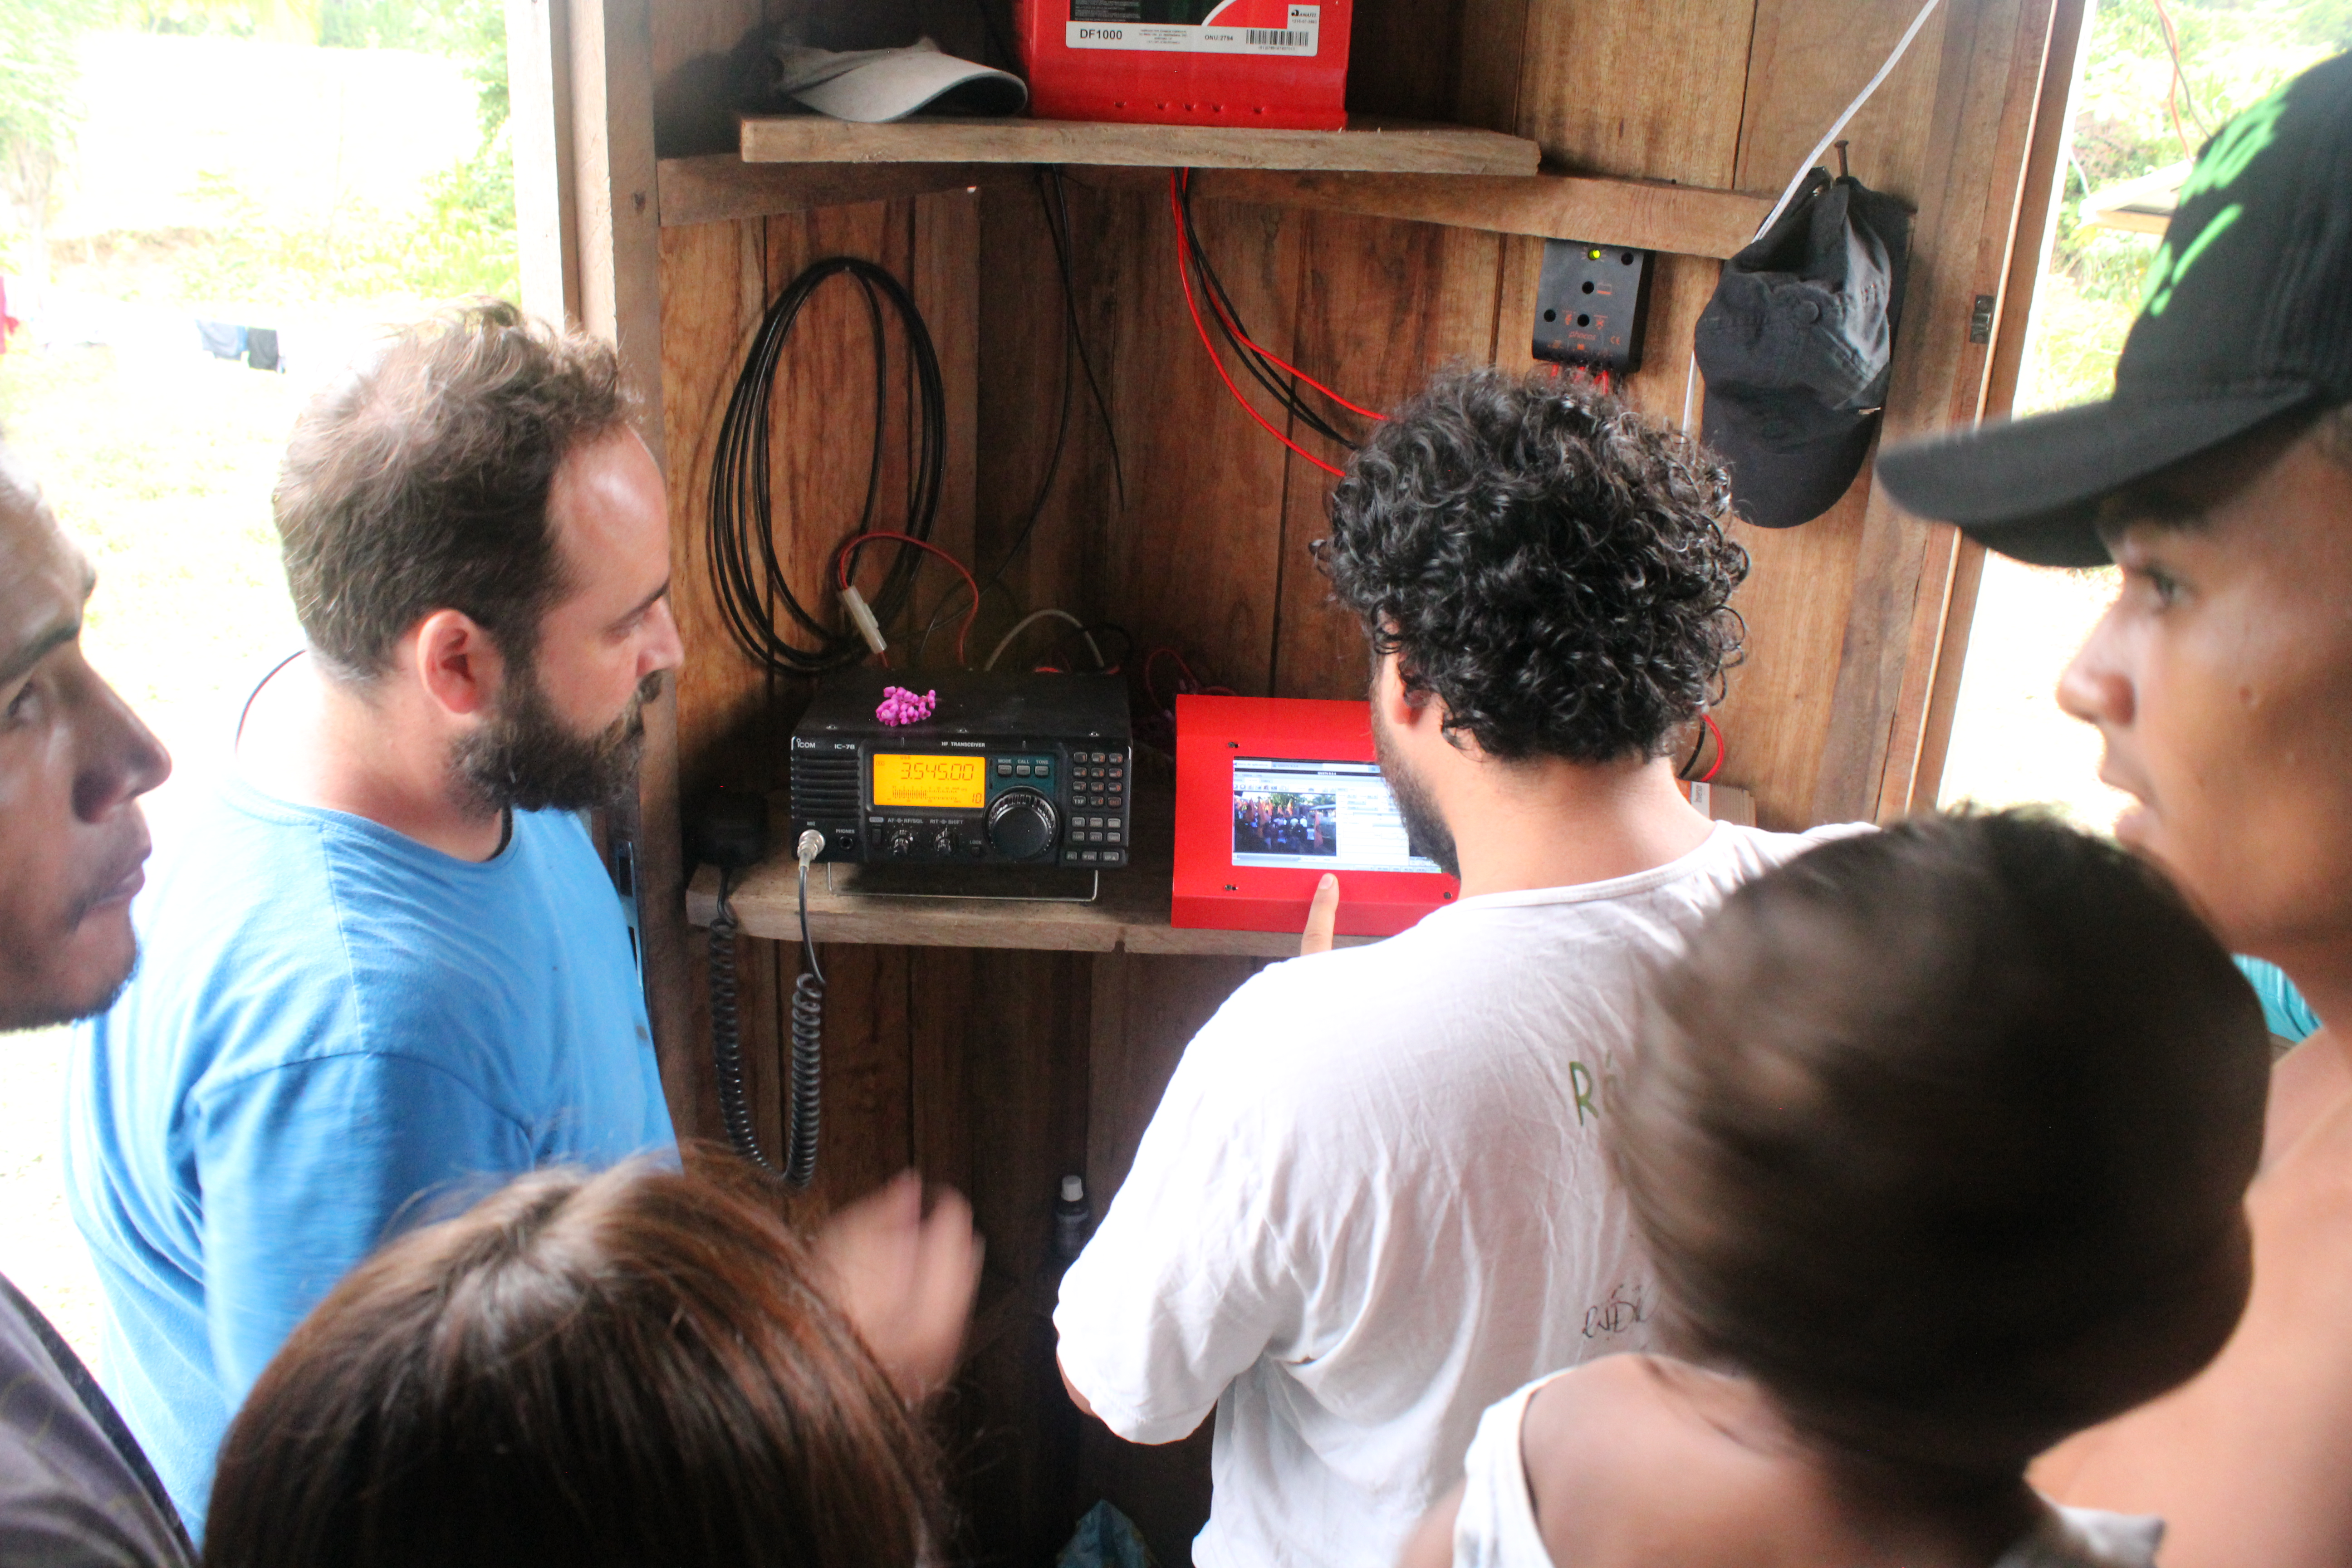
\includegraphics[width=.7\columnwidth]{radio_fonias.jpg}
  %  \includegraphics[width=.45\columnwidth]{boat.jpg}
\end{center}

\end{frame}


\begin{frame}{HERMES History}

  \begin{itemize}
    \item HERMES v1 (2018-2020): Rhizomatica's developed integrated Digital HF solution. One box includes the HF transceiver (a customized µBitx) connected to a computer. Modem used is Ardop or VARA, transport system is UUCP.
  \end{itemize}

  \includegraphics[width=.4\columnwidth]{pic3.jpg} \includegraphics[width=.49\columnwidth]{hermes2.jpeg}

\end{frame}


\begin{frame}{HERMES History}

  \begin{itemize}
  \item HERMES v1.1 (2021-2022): HF Transceiver with integrated GPS for accurate time and PLL frequency syntesis and redesigned lambda bridge.
   Improved email compression. Focus on email service and the use of DeltaChat at communities.
  \end{itemize}

%    \begin{center}

\begin{center}
%  \vspace{-0.5cm}
  \includegraphics[width=.41\columnwidth]{hermes2.jpg}
  %\includegraphics[width=.48\columnwidth]{hermes-back.jpeg}
  \includegraphics[width=.48\columnwidth]{hermes3.jpg}

%  \includegraphics[width=.45\columnwidth]{boat.jpg}
\end{center}

\end{frame}


\begin{frame}{HERMES History}

  \begin{itemize}
  \item HERMES v1.x (2019-2023): Workshops and deployments in Amazon region.
  \item HERMES v2 (2023-): Workshops and ongoing first deployment in Central Africa.
  \end{itemize}

\begin{center}
  \includegraphics[width=.3\columnwidth]{hermes4.jpeg}
  \includegraphics[width=.58\columnwidth]{foto-ecu.jpg}
\end{center}

\end{frame}

\begin{frame}{HERMES History}

  \begin{itemize}
  \item HERMES v2 (2023-): Adopted another open source wideband HF transceiver: the sBitx. Much reduced size and has native voice support (mic+ptt+speaker). Development ongoing of the Mercury modem
    for high-speed wideband capability.
  \end{itemize}

\begin{center}
  \includegraphics[width=.7\columnwidth]{sbitx1.jpeg}
\end{center}

\end{frame}

\begin{frame}{HF Telecommunication}

\begin{block}{HF Network Stack}
    \begin{itemize}
    \item Channelization: ``old'' analog-world framework (3 kHz bw), plus support to wider channels, channel aggregation and smart channel allocation
    \item Wideband HF transceicer
    \item Layer 1 (modem): all waveform, modes and bandwidths.
    \item Layer 2 (datalink): framing, Automatic Repeat reQuest (ARQ), Media Access Control (MAC)
    \item UUCP, IP, other network / transport layer
    \item Store-and-forward services (eg. email, sensors data)
    \item Voice (mobile telephony) and messaging services
    \item A tutorial on frequency adaptive communication systems in the HF bands, ITU-R, 2022 https://www.itu.int/pub/R-HDB-64-2022
    \end{itemize}
  \end{block}

\end{frame}

\begin{frame}{Real-world network example}

  \begin{itemize}
  \item In the Amazon rainforest regin, Pará state, northern Brazil
  \end{itemize}

\begin{center}
  \includegraphics[width=.57\columnwidth]{radio_stations.png}
\end{center}

\end{frame}


\begin{frame}{HERMES system features}

  \begin{itemize}
    \item Station equipment (sBitx) contains a HF transceiver and a Raspberry Pi 4
    \item UUCP based telecommunication over HF
    \item Users access HERMES services over WiFi (AP exposed by the equipment)
    \item BBS-like direct ``station-to-station'' messages (audio and image supported!)
%    \item Email is the main service, but any kind of digital data can be exchanged, as remote command execution, sensors data, etc.
    \item Email is the main service. Emails are highly compressed before going over the air
    \item Emails are synchronized to a ``gateway'' node over HF, which routes emails among HF nodes or the Internet
  \end{itemize}

\end{frame}


\begin{frame}{User interface - WEB Frontend}

\begin{block}{https://github.com/Rhizomatica/hermes-gui}
  \begin{itemize}
  \item Provides users Web access to configurations
  \item User management for both Web UI and email
  \item Multi-language: en, es, pt, fr
  \item Message system (BBS like)
  \item System logs, UUCP queue management
  \item UI for voice communication with easy frequency and mode (USB, LSB) selection and volume adjustment
  \end{itemize}
\end{block}

\end{frame}

\begin{frame}{User interface - WEB Frontend}

  \vspace{-0.15cm}
  \begin{center}
    \includegraphics[width=.9\columnwidth]{hermes-ui2.jpg}

    %    \includegraphics[width=.245\columnwidth]{gui1.png}
%    \includegraphics[width=.245\columnwidth]{gui2.png}
%    \includegraphics[width=.245\columnwidth]{gui-3.png}
%    \includegraphics[width=.245\columnwidth]{gui-4.png}

  \end{center}


\end{frame}

\begin{frame}{User interface - WEB Frontend}

  \vspace{-0.15cm}
  \begin{center}
    \includegraphics[width=.6\columnwidth]{hermes-ui3.jpg}
  \end{center}


\end{frame}


\begin{frame}{User interface - WEB Frontend}

  \vspace{-0.15cm}
  \begin{center}
    \includegraphics[width=.9\columnwidth]{hermes-ui5.jpg}
  \end{center}


\end{frame}


\begin{frame}{User interface - WEB Frontend}

  \vspace{-0.15cm}
  \begin{center}
    \includegraphics[width=.9\columnwidth]{hermes-ui4.jpg}
  \end{center}

\end{frame}


\begin{frame}{User interface - WEB Frontend}

  \vspace{-0.15cm}
  \begin{center}
    \includegraphics[width=.9\columnwidth]{hermes-ui6.jpg}
  \end{center}

\end{frame}

\begin{frame}{User interface - Analog Voice Telephony}

  \vspace{-0.15cm}
  \begin{center}
    \includegraphics[width=.9\columnwidth]{hermes5.jpeg}
  \end{center}

\end{frame}


\begin{frame}{E-mail}

\begin{block}{E-mail stack}
  \begin{itemize}
  \item E-mail software (Postfix, Dovecot) run in HERMES radio
  \item E-mail compression using uuxcomp called directly from postfix (!crmail), many headers stripped, xz compression
  \item Specific transcoding for audio (LPCNet) and image (VVC) attachments at uuxcomp
  \item One station (called ``gateway'') routes the emails between HF nodes and a main email server with public IP address (for routing over the Internet)
  \item DeltaChat is the recommended email client
  \end{itemize}
\end{block}

\vspace{-0.15cm}
\begin{center}
%    \includegraphics[width=.245\columnwidth]{gui-4.png}

\end{center}


%% add DC pictures here

\end{frame}

\begin{frame}{DeltaChat}


\begin{center}
  \includegraphics[width=.21\columnwidth]{dc1.jpg}
  \includegraphics[width=.21\columnwidth]{dc2.jpg}
  \includegraphics[width=.56\columnwidth]{webxdc.jpg}
\end{center}

\end{frame}


\begin{frame}{REST Backend}

\begin{block}{https://github.com/Rhizomatica/hermes-api}
    \begin{itemize}
    \item Radio API: set/get frequency, mode, power levels, volume, swr protection trigger, etc
    \item User API: user management for web admin access and e-mail accounts (same login)
    \item Messages API: direct message between hosts (just a uucp copy of a packaged message)
    \item System API: set/get system status / configuration
    \item UUCP API: provides a way to list and delete UUCP jobs, and start a connection (uucico)
    \item Gateway API: provides scheduling facitities and station/frequency table
    \end{itemize}
  \end{block}

\end{frame}


\begin{frame}{Good ol' UUCP}

\begin{block}{Taylor's UUCP goes over the air}
    \begin{itemize}
    \item UUCPD bridges UUCP to HF modem through pipes and shared memory
    \item The UUCP nodename is the station callsign
    \item Protocol 'y' is used, and long timeouts are set
    \end{itemize}

\vspace{0.5cm}
/etc/uucp/port:
\vspace{0.5cm}

port HFP
\\
type pipe\\
command /usr/bin/uuport -c \textbackslash Z


\end{block}


\end{frame}

\begin{frame}{HERMES-specific network stack components (hermes-net repo)}

\begin{block}{https://github.com/Rhizomatica/hermes-net}
    \begin{itemize}
    \item trx\_v1-\{firmware,userland\}: HERMES v1 transceiver firmware and radio control tools
    \item trx\_v2-userland: HERMES v2 control and DSP software for the sBitx radio
    \item uucpd: UUCP daemon and tools (bridges UUCP and the HF modem)
    \item uuxcomp: uux wrapper which compresses an e-mail before enqueuing it, and crmail to decompress
    \item system\_scripts: image and audio compression scripts, email and uucp management, gateway ``caller'', etc
    \item system\_services: init scripts and udev rules
    \end{itemize}
  \end{block}

\end{frame}


\begin{frame}{SDR Modem}
\begin{block}{Currently using VARA HF}
    \begin{itemize}
    \item 2300 Hz BW, ARQ, Adaptive Modulation
    \item Modes range from 16 bps up to 5 kbps
    \item Proprietary Visual Basic 6 application (runs well on Hangover-Wine)
    \end{itemize}
  \end{block}

\begin{center}
  \vspace{-0.15cm}\includegraphics[width=.42\columnwidth]{vara.png}
\end{center}
\end{frame}



\begin{frame}{SDR Modem}

\begin{block}{Mercury https://github.com/Rhizomatica/mercury}
    \begin{itemize}
    \item Open source configurable software-defined modem (layers 1 and 2)
    \item Modulation BPSK, QPSK, 8QAM, 16QAM, 32QAM and 64QAM
    \item LDPC code rate 2/16, 8/16 and 14/16
    \item ARQ and adaptive modulation to address different propagation conditions
    \end{itemize}
\end{block}
\vspace{-0.25cm}
  \begin{center}
    \includegraphics[width=.54\columnwidth]{image_modems.png}
  \end{center}

\end{frame}


\begin{frame}{Mercury}

  \begin{center}
    \includegraphics[width=.95\columnwidth]{mercury1.jpg}
  \end{center}

\end{frame}

\begin{frame}{Mercury Data-Link Layer}

  \begin{center}
    \includegraphics[width=.95\columnwidth]{mercury2.jpg}
  \end{center}

\end{frame}

\begin{frame}{Mercury Physical Layer}

  \begin{center}
    \includegraphics[width=.95\columnwidth]{mercury3.jpg}
  \end{center}

\end{frame}


\begin{frame}{Other characteristics}

  \begin{itemize}
  \item Robust (and stealth!) operation with 0db or less of SNR for signal reception
  \item Integration to SMS and other messaging services (https://github.com/Rhizomatica/hermes-messaging/)
  \item Sensors data acquisition and transmission - binary data using paq8px compression (https://github.com/Rhizomatica/hermes-sensors/)
  \item Support for large scale and affordable deployments
  \end{itemize}
\end{frame}

\begin{frame}{Steps for the realization of the WWWAN}

  \begin{itemize}
  \item Antenna miniaturization (nano tubes, micro strips?)
  \item Develop more advanced ML-based audio and image codecs
  \item NNCP instead of UUCP for improved security?
  \item Reticulum?
  \item Multiple users capability MAC
  \item Adaptive bandwidth and channels selection
  \item Support for real-time messaging
  \item Digital Mobile Telephony for HF
  \item DRM reception
  \item DRM broadcast
  \end{itemize}

\end{frame}

\begin{frame}{Let's Build a Global Autonomous World-Wide Area Network?}

\begin{center}
  \includegraphics[width=.2\columnwidth]{mobile.png}
  \includegraphics[width=.79\columnwidth]{mobile2.png}

\end{center}


\end{frame}


% \begin{frame}{Let's Build a Global Autonomous World-Wide Area Network?}

%\begin{center}
%  \includegraphics[width=.85\columnwidth]{picosmo.png}
%  \includegraphics[width=.79\columnwidth]{mobile2.png}
%\end{center}


%\end{frame}


% Thank you
\begin{frame}
\centering
\includegraphics[width=.5\textwidth]{multiling-TQ}
\bigskip
\begin{tabular}{cl}
\multirow{3}{*}{\huge Questions?} & \textcolor{blue}{\url{rafael@rhizomatica.org}} \\
\end{tabular}

\end{frame}

\end{document}
